
\documentclass[10pt,fleqn, twocolumn]{IEEEtran}
\usepackage{amsfonts}
\usepackage{amsthm}
\usepackage{amssymb}
\usepackage{amsmath}
\usepackage{graphicx}
\usepackage{fancyhdr}


\newtheorem{Prop}{Proposition}
\newtheorem{lemma}{Lemma}
\newtheorem{theorem}{Theorem}

\setlength{\parindent}{3em} \setlength{\oddsidemargin}{0in}
\setlength{\textwidth}{6.5in} % sets 1in left and right margins
\setlength{\topmargin}{0.20in} % change to 0.2in for regular latex
%\setlength{\headheight}{0in}
%\setlength{\footheight}{0.5in}
\setlength{\footskip}{0.5in}
\setlength{\textheight}{9.0in} %sets 1in top and bottom margins
\renewcommand{\baselinestretch}{1} %set to 1.5 for double spacing.

\newcommand{\br}{{\mathbf r}}
\newcommand{\bA}{{\mathbf A}}
\newcommand{\ba}{{\bf a}}
\newcommand{\bb}{{\bf b}}
\newcommand{\bc}{{\bf c}}
\newcommand{\bC}{{\bf C}}
\newcommand{\bd}{{\bf d}}
\newcommand{\be}{{\bf e}}
\newcommand{\bE}{{\bf E}}
\newcommand{\bbf}{{\bf f}}
\newcommand{\bF}{{\bf F}}
\newcommand{\bh}{{\bf h}}
\newcommand{\bH}{{\bf H}}
\newcommand{\bg}{{\bf g}}
\newcommand{\bG}{{\bf G}}
\newcommand{\bq}{{\bf q}}
\newcommand{\bs}{{\bf s}}
\newcommand{\bm}{{\bf m}}
\newcommand{\bn}{{\bf n}}
\newcommand{\bu}{{\bf u}}
\newcommand{\bv}{{\bf v}}
\newcommand{\bw}{{\bf w}}
\newcommand{\bx}{{\bf x}}
\newcommand{\by}{{\bf y}}
\newcommand{\bz}{{\bf z}}
\newcommand{\bL}{{\bf L}}
\newcommand{\bM}{{\bf M}}
\newcommand{\bN}{{\bf N}}
\newcommand{\bS}{{\bf S}}
\newcommand{\bT}{{\bf T}}
\newcommand{\bD}{{\bf D}}
\newcommand{\bX}{{\bf X}}
\newcommand{\bP}{{\bf P}}
\newcommand{\bQ}{{\bf Q}}
\newcommand{\bI}{{\bf I}}
\newcommand{\bR}{{\bf R}}
\newcommand{\bU}{{\bf U}}
\newcommand{\bV}{{\bf V}}
\newcommand{\bW}{{\bf W}}
\newcommand{\bY}{{\bf Y}}
\newcommand{\bZ}{{\bf Z}}
\newcommand{\bJ}{{\bf J}}
\newcommand{\bB}{{\bf B}}
\newcommand{\bzero}{{\bf 0}}
\newcommand{\bgamma}{{\mbox {\boldmath $\gamma$}}}
\newcommand{\btheta}{{\mbox {\boldmath $\theta$}}}
\newcommand{\bvartheta}{{\mbox {\boldmath $\vartheta$}}}
\newcommand{\bDelta}{{\mbox {\boldmath $\Delta$}}}
\newcommand{\bLambda}{{\mbox {\boldmath $\Lambda$}}}
\newcommand{\bPsi}{{\mbox {\boldmath $\Psi$}}}
\newcommand{\bPhi}{{\mbox {\boldmath $\Phi$}}}
\newcommand{\bcA}{{\mbox {\boldmath ${\cal A}$}}}
\newcommand{\bcB}{{\mbox {\boldmath ${\cal B}$}}}
\newcommand{\bcC}{{\mbox {\boldmath ${\cal C}$}}}
\newcommand{\bcD}{{\mbox {\boldmath ${\cal D}$}}}
\newcommand{\bcF}{{\mbox {\boldmath ${\cal F}$}}}
\newcommand{\bcG}{{\mbox {\boldmath ${\cal G}$}}}
\newcommand{\bcL}{{\mbox {\boldmath ${\cal L}$}}}
\newcommand{\bcN}{{\mbox {\boldmath ${\cal N}$}}}
\newcommand{\bcR}{{\mbox {\boldmath ${\cal R}$}}}
\newcommand{\bcS}{{\mbox {\boldmath ${\cal S}$}}}
\newcommand{\bcH}{{\mbox {\boldmath ${\cal H}$}}}
\newcommand{\bcI}{{\mbox {\boldmath ${\cal I}$}}}
\newcommand{\bcO}{{\mbox {\boldmath ${\cal O}$}}}
\newcommand{\bcP}{{\mbox {\boldmath ${\cal P}$}}}
\newcommand{\bcQ}{{\mbox {\boldmath ${\cal Q}$}}}
\newcommand{\bcV}{{\mbox {\boldmath ${\cal V}$}}}
\newcommand{\bcW}{{\mbox {\boldmath ${\cal W}$}}}


\title{On The Reliability of MIMO Beamforming Feedback Channel}
\author{\\LG Electronics Mobile Research\\San Diego, CA 92131-1807}
\date{}
\begin{document}
\maketitle
\begin{abstract}\small
The reliability of the feedback channel for MIMO beamforming is
investigated in this paper. We model MIMO beamforming feedback by
a noisy Gaussian binary erasure feedback channel, in which the
MIMO forwardlink is modelled as a Gaussian channel and the
reverselink is simplified as a Gaussian binary erasure channel.
For forwardlink channel estimation, Cramer-Rao lower bound is
derived for time-multiplexing pilot pattern and superimposed
pilots, respectively. For reverselink transmission, a Hamming
bound for codebook design is given. The reliability of MIMO
feedback channel is analysis and derived after these. When the
MIMO feedback rate is less than a certain threshold, it shows that
the feedback channel reliability is mostly decided by the feedback
channel erasure rate. However, the rate threshold is controlled by
forwardlink channel design, reverselink channel condition and
codebook design.

\end{abstract}
\section{Introduction}
Multi-antenna systems have received much attention over the last
decades, due to their promise of higher spectrum efficiency with
no transmit power increase. For multiple-input multiple-output
(MIMO) transmission, it is well-known that the retransmission
delay, reliability and complexity can be improved by making
channel state information (CSI) available at the transmitter side.
This is usually achieved through a reverselink CSI feedback
channel from receiver. In practice, the CSI received by the
transmitter is imperfect and suffers from various impairments
including round-trip delay, channel estimation error, codebook
limitation, etc. It results that the actual forwardlink throughput
is degraded.

MISO/MIMO beamforming systems with ideal Lloyd vector quantization
(VQ)~\cite{Narula98}, different channel model~\cite{Mukka03} or
different performance metrics~\cite{PXia04,Roh04} were discussed.
However, most of them are done without considering the effects of
"noisy" feedback including forwardlink pilot design and channel
estimation, even though they are among the most important
components of actual multi-antenna systems. In reality, MIMO CSI
is estimated with forwardlink common pilot channels sent from each
transmitter antenna. An overview of pilot-assisted transmission
(PAT) including pilot placement and channel estimation can be
found in~\cite{Tong04}. In most multi-antenna systems, pilot
channels are designed to be orthogonal to other channels and
periodically sent by transmitter. Nonorthogonal pilot design like
superimposed pilots (SIP) has recently received much attention for
channel estimation too~\cite{Coldrey06}. Optimal pilot placement
was investigated in~\cite{Dong02}. The feedback channel capacity
are investigated over decades~\cite{Shannon56,Kim06}. Though
feedback doesn't increase the capacity of memoryless channels, the
decoding error probability of a proper feedback scheme may
decrease more rapidly than the exponential of any
order~\cite{Kramer69} in addition to the help of simplifying
transceiver design. In practical system design, it is important to
understand the reliability of feedback channel and therefore
system throughput with finite-rate feedback.

In this paper, the reliability of MIMO feedback channel is
discussed with considering forwardlink design and reverselink
channel condition. The forwardlink for channel estimation is
modelled as a Gaussian channel with pilot and data signals
transmitted. On MIMO forwardlink design, the Cramer-Rao lower
bound (CRLB) of channel estimation is analyzed and presented,
respectively, for time-multiplexed pilots (TMP) or SIP. The MIMO
feedback channel in reverselink is modelled as a binary erasure
channel with additive Gaussian noise. The binary erasure channel
is a popular model for fading channel, especially for reverselink
feedback channels. The additional Gaussian noise is for the
channel background noise and channel quantization errors of
reverselink. With this noisy Gaussian binary erasure channel
model, some results regarding the feedback channel reliability can
be straightforwardly obtained. It shows that when the reverselink
feedback rate is under a certain threshold, the channel
reliability is mostly decided by the reverselink erasure rate,
where the reverselink feedback rate is a function of the shared
codebook size and feedback period. On the other hand, the feedback
threshold is decided by forwardlink design, reverselink channel
condition and codebook design.

\section{System Model And Problem Description\label{MIMO_system_model}}

Consider a MIMO link consisting of a transmitter with $M$ transmit
antennas, a receiver with $N$ receive antenna and a MIMO channel
represented by the $N\times M$ matrix $\bH=\left[\bh_{1}\ \bh_{2}\
\ldots\ \bh_{N}\right]^{\rm T}$ with $\bh_{n}=\left[h_{n,1}\
h_{n,2}\ \ldots\ h_{n,M}\right]^{\rm T}$ . The $N\times 1$
received signal $\by$ is
\begin{equation}
\begin{array}{rcccl}
\by&=&\left[y_{1}\ y_{2}\ \ldots\ y_{N}\right]^{\rm T}& = &
\bH\bW\bx+\bn
\end{array}\label{Direct_MIMO}
\end{equation}
\noindent where $\bx=\left[x_{1}\ x_{2}\ \ldots\ x_{M}\right]^{\rm
T}$ is the $M\times 1$ signal vector transmitted by the source
with $\bR_{\bx}=\mbox{E}\left\{\bx\bx^{\rm
H}\right\}=\frac{P}{M}\bI_{M}$, $P$ is the total transmit power,
$\bW=\left[\bw_{1}\ \bw_{2}\ \ldots\ \bw_{M}\right]$ is a $M\times
M$ MIMO beamforming precoding matrix with
$\left\|\bw_{m}\right\|_2=1$, $\bn\sim{\bcC\bcN}(0,
\sigma^2\bI_{N})$ is a complex circular white Gaussian vector,
$\left[\ast\right]^{\rm T}$ and $\left[\ast\right]^{\rm H}$
denotes the transpose operator and Hermitian conjugate operator,
respectively. The MIMO channel achievable spectral efficiency is
\begin{equation}\hspace{-0.14in}
\begin{array}{l}
\eta=\log\left|\bI+\frac{P}{M}\bH\bW\bW^{\rm H}\bH^{\rm H}\right|=
\sum\limits_{k=1}^{K}\log\left(1+\frac{\rho_{i}}{M}\right)
\end{array}\label{spectral_eff}
\end{equation}
\noindent where $\rho_{i}$ denotes the received signal-to-noise
ratio (SNR) of the $k$th beam, which is given by
\begin{equation}
\begin{array}{rcccl}
\rho_{i}&=&\frac{\mbox{var}\left\{\bH\bw_{i}x_{i}\right\}}{\sigma^2}&=&\frac{\lambda_{i}P_{i}}{\sigma^2}
\end{array}\label{SNR_i}
\end{equation}
\noindent with $\lambda_{i}$ denoting the antenna gain of the
$i$th beam and also the $i$th eigenvalue of the MIMO channel
autocorrelation matrix $\bR_{\bH}$ defined by
\begin{equation}
\begin{array}{l}
\bR_{\bH}=\bH^{\rm H}\bH=\sum\limits_{m=1}^{M}\bh_{m}\bh_{m}^{\rm
H}=\sum\limits_{i=1}^{M}\lambda_{i}\bv_{i}\bv_{i}^{\rm H}
\end{array},\label{R_h}
\end{equation}
\noindent $\bv_{i}$ denotes the $i$th eigenvector, the operator
$\left|\ast\right|$ denotes the determinant of matrix $\ast$, and
$\mbox{var}\left\{\ast\right\}$ denotes the variance of random
variable $\ast$. (\ref{spectral_eff}) and (\ref{SNR_i}) are the
results from the assumption of perfect CSI available at
transmitter, however this may not be consistent with practical
applications.

In reality, the receivers estimate $\bH$ or $\bR_{\bH}$ with the
pilots sent by transmitter at first. Accuracy of the channel
estimation depends on forwardlink design. There are two popular
forwarlink data/pilot patterns, TMP and SIP, receiving much
attention for MIMO channel estimation. After channel estimation,
receiver will choose a beamforming vector from a shared MIMO
precoding codebook. This is called channel quantization. And
receiver then feeds back the chosen precoding index(es) to
transmitter(s) instead of actual channel response for the next
transmit precoding. With a MIMO codebook $\bcW$ of the size $2^B$
consisting of $M$-dimensional normalized vectors $\left\{\bw_{1},
..., \bw_{2^{B}}\right\}$, it takes the receiver to feedback $B$
bits for each beam stream. A codebook is usually designed to
quantize channel responses with certain distortion
measures~\cite{Narula98}. This is related to Grassmannian line
packing and the spherical packing on unit sphere
$\bcS_{n}\left(1\right)$~\cite{Love02}, where
$\bcS_{n}(R)=\left\{\bv:\ \left\|\bv\right\|=R\right\}$ denotes
$(n-1)$-sphere of radius $R$. When a codeword $\bw_k$ is chosen to
precode transmit signals for $i$th beam $\bv_{i}$ at the
transmitter side, some degradation will usually happen on the
signals received by receiver because of imperfect channel
estimation and finite-rate feedback. This degradation on received
signals can be expressed by
\begin{equation}
\begin{array}{rcl}
\delta_{i} & = & \min\limits_{\bw\in\bcW}\left\|\bH\bv_{i}-\bH\bw\right\|\\
&=&\lambda_{i}\left(1-\bv_{i}^{\rm
H}\bw_k\right)-\sum\limits_{j\neq i}\lambda_{j}\bv_{j}^{\rm
H}\bw_{k}
\end{array}\label{delta_i}
\end{equation}
\noindent where $\bv_{i}$ is the ideal precoding vector for $i$th
eigen-mode of $\bH$. It is known that $\delta_{i}$ is one of the
major factors limiting closed-loop MIMO beamforming throughput,
which depends on $\bv_{i}$, $\bw_{k}$ and $\lambda_{i}$, etc.

\begin{figure}
\center{
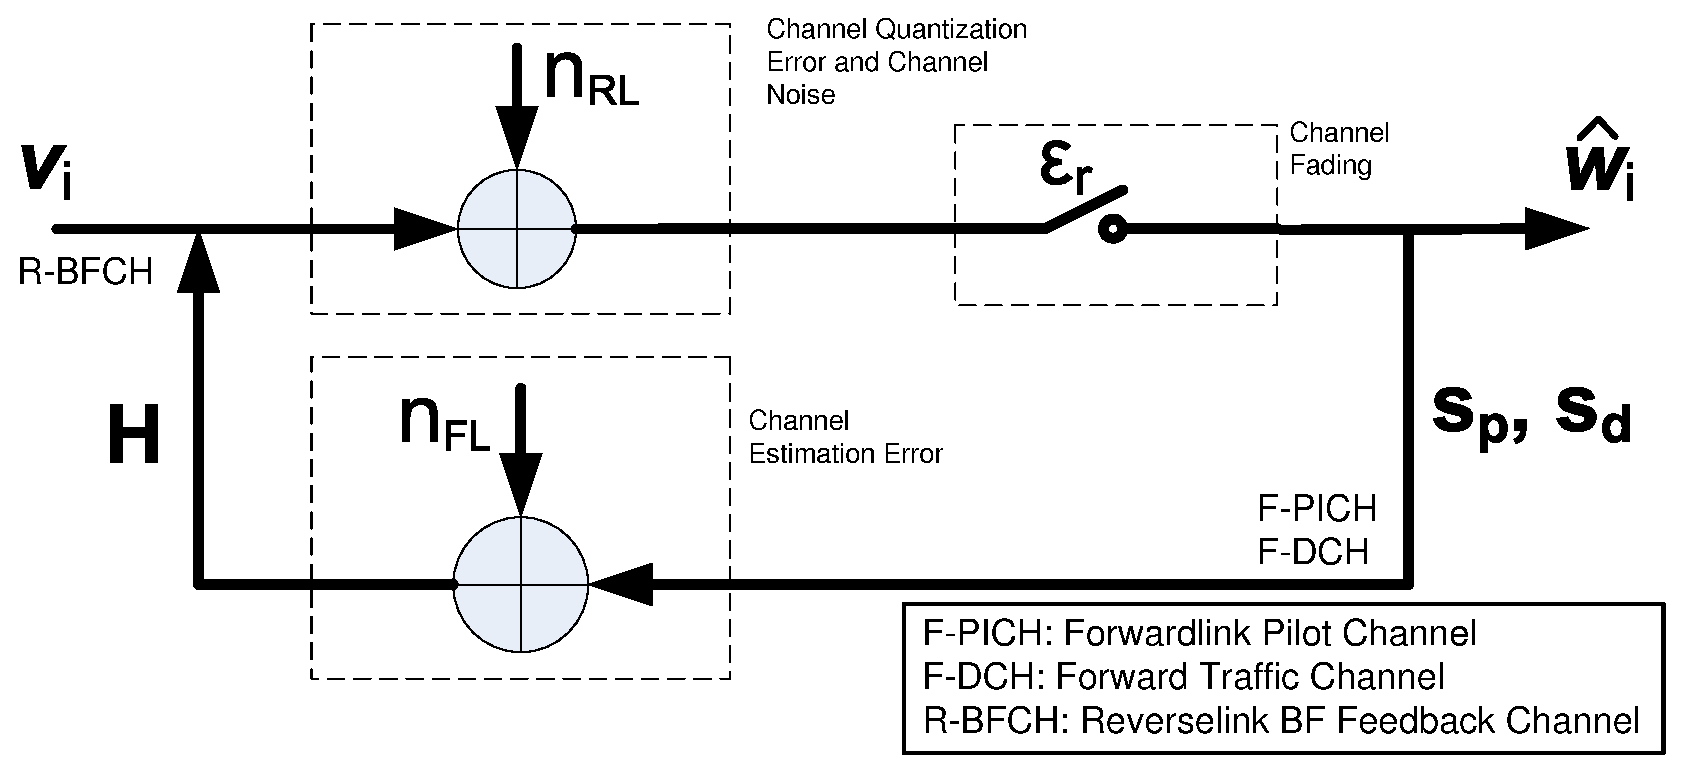
\includegraphics[width=3.0in, angle=0]{Noisy_Gaussian_Feedback_Channel.eps}
\caption{Noisy Gaussian binary erasure feedback
channel.}\label{noisy_Gaussian_feedback} }
\end{figure}

Alternatively, the above description of MIMO beamforming with
finite-rate feedback can be modelled as a noisy Gaussian binary
erasure feedback channel depicted in
Fig.~\ref{noisy_Gaussian_feedback}. In the noisy Gaussian binary
erasure feedback channel model, the receiver side feedbacks actual
channel information $\bH$ through a Gussian channel to the
transmitter side, in which the Gaussian variable $n_{\rm FL}$
denotes channel estimation errors.  The transmitter side then
estimates the channel $\bH$, quantizes it and sends it to the
received side through a Gaussian binary erasure channel, in which
the Gaussian variable $n_{\rm RL}$ denotes the sum of the additive
background Gaussian channel interfernece/noise and quantization
errors and $\varepsilon_{\rm r}$ denotes the erasure rate due to
channel fading. For reverselink feedback channel design, we are
interested in both the achievable rate and the associated
reliability. This is the region of achievable rate distortion pair
$\left(R,\ \epsilon\right)$, where $\epsilon$ is the error
exponent denoting how fast the reverselink bit-error rate (BER)
$P_{e}$ decays for the transmit rate $R$ and it can be expressed
by

\begin{equation}
\begin{array}{rcccl}
\epsilon&=&\lim\limits_{n\rightarrow\infty}\sup
\epsilon_{n}&=&\lim\limits_{n\rightarrow\infty}\sup-\frac{1}{n}\ln
P_{e}
\end{array}
\end{equation}

\noindent where $\epsilon_{n}=-\frac{1}{n}\ln P_{e}$ denotes the
reliability of $n$-bits block transmission and $n$ is the minimum
block-length needed in order to operate at rate $R$ with the error
probability $P_{e}$. In the following sections, we will discuss
how the imperfect channel estimation affect the reliability of
MIMO feedback channel and therefore forwardlink throughput.

\section{The Feedback Channel Noises}

\subsection{Channel Estimation Errors $n_{\rm FL}$}

\begin{figure}
\center{
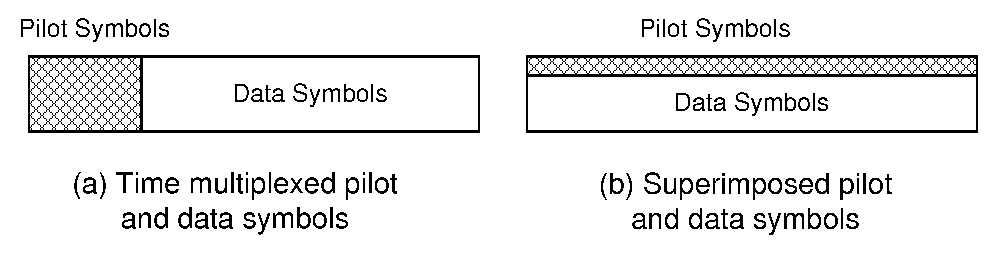
\includegraphics[width=3in, angle=0]{Pilot_Patterns.eps}
\caption{Pilot patterns for channel
estimation.}\label{pilot_pattern} }
\end{figure}

In general, the channel estimation model for frequency-selective
block fading channel is different to (\ref{Direct_MIMO}). For
practical channel estimation, not only the whole channel impulse
response but also the pilot placement should be considered.
Considering a $M$-input/$N$-output MIMO channel with
frequency-selective block fading, which means the random channels
taps remain constant for some data packets and change to
independent values for the next block, the received baseband
signal can be written by
\begin{equation}\hspace{-0.20in}
\begin{array}{rcl}
\by&=&\left[\begin{matrix}y_{1}(t)&y_{2}(t)&\cdots&y_{N}(t)\end{matrix}\right]^{\rm T}\\
&=&\left[\begin{matrix}\sum\limits_{m=1}^{M}h_{m,1}(t)\otimes s_m(t)\\ \sum\limits_{m=1}^{M}h_{m,2}(t)\otimes s_m(t)\\ \vdots \\
\sum\limits_{m=1}^{M}h_{m,N}(t)\otimes
s_m(t)\end{matrix}\right]+\left[\begin{matrix}n_{1}(t)\\ n_{2}(t)\\ \vdots\\
n_{N}(t)\end{matrix}\right]\\
&=&\bS\bh+\bn
\end{array}
\end{equation}
\noindent where $s_m(t)$ denotes the transmitted symbol from the
$m$th antenna, $\bh$ is the stretched channel vector defined by
\begin{equation}\hspace{-0.00in}
\begin{array}{rcl}
\bh&=&\mbox{vec}\left(\left[\mbox{vec}(\bH_{1})\
\mbox{vec}(\bH_{2})\ \ldots\ \mbox{vec}(\bH_{N})\right]\right)
\end{array}
\end{equation}
\noindent with $\bH_{n}=\left[\bh_{n}(0)\ \bh_{n}(1)\ \ldots\
\bh_{n}(L_{c}-1)\right]$, $\bh_{n}(l)=\left[h_{n,1}(l)\
h_{n,2}(l)\ \ldots\ h_{n,M}(l)\right]^{\rm T}$ for $1\leq l \leq
L_{c}$, and
\begin{equation}\hspace{-0.00in}
\begin{array}{rcl}
\bS&=&\mbox{kron}\left(\left[\bS_{1}\ \bS_{2}\ \ldots\
\bS_{M}\right]^{\rm T},\ \bI\right)
\end{array}
\end{equation}
\noindent with
\begin{equation}\hspace{-0.10in}
\begin{array}{rcl}
\bS_{k}&=&\left[\begin{matrix}
s_{k}(L)&\cdots&s_{k}(L-L_{c})\\
s_{k}(L-1)&\cdots&s_{k}(L-L_{c}-1)\\
\vdots&\ddots&\vdots\\
s_{k}(1)&\cdots&s_{k}(1-L_{c})
\end{matrix}\right]
\end{array}.\label{S_k}
\end{equation}
\noindent $L_{c}$ is the maximum channel order for all
subchannels. After the channel response vector $\bh$ is estimated,
we can calculate the channel correlation matrix $\bR_{\bH}$ by
\begin{equation}\hspace{-0.1in}
\begin{array}{rcl}
\hat{\bR}_{\bH}&=&\frac{1}{L_{c}}\sum\limits_{l=1}^{L_{c}}\sum\limits_{n=1}^{N}\hat{\bh}_{n}\left(L_{c}+l\right)\hat{\bh}_{n}^{\rm
H}\left(L_{c}+l\right)
\end{array}.\label{R_h_actual}
\end{equation}

There are many ways to put pilot symbols and data symbols together
for PAT. We focus on two most popular designs: an {orthogonal
design} by {time-multiplexed pilot pattern}, and a {non-orthogonal
design} by {superimposed pilot pattern}, in this paper. TMP is a
typical example of orthogonal pilot design where pilot symbols and
data symbols are separated in time and/or frequency domain, which
makes them orthogonal to each other. With orthogonal pilots, the
channel estimation and data demodulation can be done separately
which may lead to simple receiver design~\cite{Dong02}. SIP does
the opposite. In SIP design, pilots and data nonorthogonally share
the same time period and frequency band. In this case, joint
channel estimation/demodulation and the demodulation with pilot
interference cancellation are among the most popular receiver
design techniques~\cite{Coldrey06}.

\subsubsection{Time-Multiplexed Pilots and Data}
The concept of TMP design is to send $Q$ known pilot symbols and
$\left(L-Q\right)$ data symbols consecutively and separately in
time domain. One possible example of TMP is shown in
Fig.~\ref{pilot_pattern}(a), in which the transmitted symbol
$s_{k}(l)$ is
\begin{equation}
\begin{array}{rcl}
s_{k}\left(l\right)&=&
\begin{cases}
s_{pk}(l) & 1 \leq l \leq Q \\
s_{dk}(l-Q) & Q+1\leq l\leq L
\end{cases}
\end{array},\label{TMP_k}
\end{equation}
\noindent where $s_{pk}(t)$, $1\leq t \leq Q$, denotes the pilot
symbols transmitted in power $\sigma_{p}^2$ and $s_{dk}(t)$,
$Q+1\leq t \leq L$, denotes the data symbols transmitted in power
$\sigma_{d}^2$.
\subsubsection{Superimposed Pilots and Data}
In SIP design, data symbols and pilot symbols are simultaneously
sent within one frame of $L$ symbols. This can be shown in
Fig.~\ref{pilot_pattern}(b). In this case, the transmitted symbol
$s_{k}(l)$ becomes
\begin{equation}
\begin{array}{rcl}
s_{k}\left(l\right)&=&\frac{\sigma_{p}}{P}s_{pk}\left(l\right)+\frac{\sigma_{d}}{P}s_{dk}\left(l\right)\
,\ 1\leq l\leq L\ ,
\end{array}\label{SIP_k}
\end{equation}
\noindent with $\sigma_{p}^2+\sigma_{d}^2=P$.

The lower bound to the mean-squared errors (MSE) of unbiased
channel estimates is given by CRLB, which is defined as the
inverse of the Fisher Information Matrix (FIM). If we denotes
$\bvartheta=\left[\bh^{\rm T}\ \bs_{d}^{\rm T}\right]^{\rm T}$,
the complex FIM is given by
\begin{equation}\hspace{-0.10in}
\begin{array}{rcl}
\mbox{F}\left(\bvartheta\right)&=&\mbox{E}\left\{\left[\frac{\partial\ln\mbox{Pr}\left(\by|\vartheta\right)}{{\partial\vartheta}^{\ast}}\right]\left[\frac{\partial\ln\mbox{Pr}\left(\by|\vartheta\right)}{{\partial\vartheta}^{\ast}}\right]^{\rm H}\right\}\\
 &\hspace{-0.90in}=&\hspace{-0.50in}\sigma_{n}^{-2}\left[\begin{matrix}
\mbox{E}\left\{\bS^{\rm
H}\bS\right\}+\rho_{h}^2\bI&\bzero\\
\bzero&\mbox{E}\left\{\bcH^{\rm H}\bcH\right\}+\rho_{s_{d}}^2\bI
\end{matrix}\right]\ ,
\end{array}\label{FIM}
\end{equation}
\noindent where
$\rho_{h}^{2}=\mbox{E}\left\{\left|\frac{\partial\ln\mbox{Pr}\left(h\right)}{{\partial
h}^{\ast}}\right|^2\right\}$ and
$\rho_{s_{d}}^{2}=\mbox{E}\left\{\left|\frac{\partial\ln\mbox{Pr}\left(s_{d}\right)}{{\partial
s_{d}}^{\ast}}\right|^2\right\}$. With (\ref{FIM}), the MSE of the
estimates of $\bR_{\bh}=\mbox{E}\left\{\bh\bh^{\rm H}\right\}$ is
given by
\begin{equation}
\begin{array}{rcl}
\mbox{MSE}\left\{\bR_{\bh}\right\}&=&\sigma_{n}^{2}\left[\mbox{E}\left\{\bS^{\rm
H}\bS\right\}+\rho_{h}^2\bI\right]^{-1}
\end{array}.
\end{equation}
\noindent The CRLB on the channel estimation with either TMP or
SIP can therefore be formulated by the following lemma.
\begin{lemma}(Cramer-Rao Lower Bound) For the time-multiplexed pilot and data design defined in
(\ref{TMP_k}), the CRLB of channel estimation is
\begin{equation}
\begin{array}{rcl}
\sigma_{\mbox{\tiny
FL}}^{2}&\geq&\left[\rho_{h}^2+Q\rho_{p}^2+\left(L-Q\right)\rho_{d}^2\right]^{-1}
\end{array}.\label{CRLB_TMP}
\end{equation}
\noindent For the superimposed pilot and data design defined in
(\ref{SIP_k}), the CRLB of channel estimation is
\begin{equation}\
\begin{array}{rcl}
\sigma_{\mbox{\tiny
FL}}^{2}&\geq&\left[\rho_{h}^2+L\left(\rho_{p}^2+\rho_{d}^2\right)\right]^{-1}
\end{array}\label{CRLB_SIP}
\end{equation}
\noindent where $\rho_{p}^2=\frac{\sigma_{p}^2}{\sigma_{n}^2}$
denotes the SNR of received pilot signals and
$\rho_{d}^2=\frac{\sigma_{d}^2}{\sigma_{n}^2}$ denotes the SNR of
received data signals.
\end{lemma}

\subsection{Channel Quantization Error}
\begin{figure}
\center{
\includegraphics[width=3.20in, angle=0]{Voronoi_Bounds2.eps}
\caption{Voronoi cell and various bounds}\label{Voronoi_bound} }
\end{figure}
It is known that the performance of channel quantization depends
on the codebook Voronoi decomposition. However, the closed-form
expression of a general Voronoi cell boundary is an open-problem
even for regular Voronoi tessellation. This makes it difficult to
obtain some insights into the average SINR and achievable
throughput for the MIMO beamforming with finite-rate feedback.
There are two other well-known open problems related to Voronoi
decomposition. The first one is called disk-covering problem in
which, given a unit disk, the problem is to find the smallest
radius for $n$ equal disks to completely cover the unit disk. The
other one is sphere-packing problem which concerns arrangements of
non-overlapping identical spheres to fill a space. The
relationship between Voronoi cell and the solutions to the
disk-covering problem and sphere-packing problem is illustrated in
Fig.~\ref{Voronoi_bound}. Basically the sphere-packing solution
gives a lower-bound approximation of Voronoi cell and the
disk-covering solution presents an upper-bound approximation of
it. The difference is measured by the parameter called {\em
packing efficiency}, which approaches $1$ when the sphere
dimension becomes large.

Instead of finding the exact boundary for the Voronoi cell
$\bcV_{i}$, we suggest a heuristic approach using Hamming bound
and sphere cap to approximate the actual polytope boundary. It
also is an approximate of the sphere packing solution, in which
all spheres are supposed to be non-overlappedly placed. With our
approach, sphere caps are overlapped with each other in space but
the interior of them has the same area as the Voronoi cell. The
border of this sphere cap is termed Hamming boundary. The
relationship between Hamming boundary and Voronoi cell is shown in
Fig.~\ref{Voronoi_bound}. For an uniform random codebook of size
$2^{B}$ in $M$-dimensional Euclid space, the area of a Voronoi
cell is given by
\begin{equation}
\begin{array}{rcl}
A\left(\bcV_{k}\right)&=&
\frac{2{\pi}^{M}}{2^{B}\Gamma\left(M\right)}
\end{array}\label{V_area}
\end{equation}
\noindent where $\Gamma\left(\ast\right)$ denotes the gamma
function. On the other hand, the area of $(m-1)$-complex sphere
cap $\bcC_{m}^{\rm c}\left(\psi,\ R\right)$ with contact angle
$\psi$ and radius $R$ is
\begin{equation}%\hspace{-0.22in}
\begin{array}{l}
A\left(\bcC_{m}^{\rm c}\left(\psi,\
R\right)\right)=\left[1-\cos^{2(m-1)}\left(\psi\right)\right]S_{m}^{\rm
c}\left(R\right),
\end{array}
\end{equation}
\noindent where ${\bcS}_{m}^{\rm c}\left(R\right)$ denotes a
$M$-dimension complex ball in Euclid space with the radius $R$.
The relationship between ${\bcS}_{m}^{\rm c}\left(R\right)$ and
$\bcC_{m}^{\rm c}\left(\psi,\ R\right)$ can be shown in
Fig.~\ref{Voronoi_bound} and it can be verified that
\begin{equation}
\begin{array}{rcl}
A\left(S_{m}^{c}\left(R\right)\right)&=&A\left(\bcC_{m}^{\rm
c}\left(\pi,\ R\right)\right)
\end{array}.
\end{equation}
\noindent With matching the sum area of the sphere-cap with the
whole sphere area, the boundary of a Voronoi cell can be
approximated by a hypershpere or a closed space curve defined in
the following proposition.
\begin{Prop}\label{approx_bound}(Hamming Boundary) The boundary of the uniform complex Voronoi cell $\bcV_{k}$ can be
approximated by a $(M-1)$-unit complex sphere or a closed complex
space curve.
\begin{equation}\hspace{-0.05in}
\begin{array}{rcl}
\bB\left(\bcV_{k}\right)&\approx& \bcS_{M}^{\rm c}(1)\bigcap \bcL_{M}^{\rm c}(\bw_{k},\ \cos(\theta)) \\
&=&\left\{\bv:\ \left\|\bv\right\|=1,\ \angle\left(\bv,\
\bw_{k}\right)=\theta\right\}\ ,
\end{array}
\end{equation}
\noindent where $\bcL_{M}^{\rm c}\left(\bw_{k},\
\cos(\theta)\right)=\left\{\bv:\ \bv^{\rm
H}\bw_{k}=\cos(\theta)\right\}$ denotes a complex space curve and
$\theta$ is
\begin{equation}%\hspace{-0.00in}
\begin{array}{rcl}
\theta&=&\arccos\left(\alpha_{0}\right)
\end{array}
\end{equation}
\noindent with
\begin{equation}\hspace{-0.00in}
\begin{array}{rcl}
\alpha_{0}&=&\left(\frac{2^B-1}{2^B}\right)^{\frac{1}{2M-2}}
\end{array}.
\end{equation}
\end{Prop}
On the other hand, if the ideal channel precoding vector $\bv_{i}$
is assumed to be a random variable of $M$-dimensional uniform
distribution, the probability density function (PDF)
$\mbox{pr}\left(\alpha\right)$ of $\alpha$ are
\begin{equation}\hspace{-0.10in}
\begin{array}{l}
\mbox{Pr}\left[x=\alpha\right]=\begin{cases}
0 & 0\leq \alpha < \alpha_{0} \\
\frac{\left(2M-2\right)\alpha\left(1-\alpha^2\right)^{M-2}}{\left(1-\alpha_{0}^{2}\right)^{M-1}}
& \alpha_{0}\leq\alpha\leq 1
\end{cases}
\end{array}
\end{equation}
\noindent and the cumulated density function (CDF) is
\begin{equation}\hspace{-0.15in}
\begin{array}{l}
\mbox{Pr}\left[x\leq\alpha\right]=
\begin{cases}
0 & 0 \leq\alpha < \alpha_{0} \\
1-\left(\frac{1-\alpha^2}{1-\alpha_{0}^2}\right)^{M-1} &
\alpha_{0}\leq\alpha\leq 1
\end{cases}\ .
\end{array}
\end{equation}
\noindent With the assumption of uniform random codebook and MIMO
channels, the average received SINR $\bar\rho_{i}$ can be
approximated by the following lemma.
\begin{lemma} A heuristic mean of $\rho_{i}$
can be expressed by
\begin{equation}%\hspace{-0.10in}
\begin{array}{rcl}
\bar\rho_{i}&\approx&\frac{\sigma_{\alpha}^{2}\rho_{i}}{1+
\left(\frac{1-\sigma_{\alpha}}{M-1}\right)^{2}\sum\limits_{j\neq
i}\frac{\lambda_{i}}{\lambda_{j}}\rho_{j}}\ ,
\end{array}
\end{equation}
\noindent where $\sigma_{\alpha}$ denotes the standard deviation
of $\alpha$ and $\sigma_{\alpha}^2$ is given by
\begin{equation}\hspace{-0.2in}
\begin{array}{rcccl}
\sigma_{\alpha}^2&=&\mbox{E}\left\{\alpha_{i}^2\right\}&=&\frac{1}{M}+\frac{M-1}{M}\left(\frac{2^B-1}{2^B}\right)^{\frac{1}{M-1}}
\end{array}.\label{sigma_alpha}
\end{equation}
\end{lemma}

\section{The Reliability of Feedback Channel}

With noiseless feedback, it is known that the reliability is
bounded by
\begin{equation}
\begin{array}{rcl}
\epsilon\left(R\right)&\leq&\bD\left(\hat{\bw}\|\bv\right)\left(1-\frac{R}{C}\right)
\end{array},
\end{equation}
\noindent where $\bD\left(p\| q\right)$ denotes the relative
entropy between two probability mass function $p\left(x\right)$
and $q\left(x\right)$ and given by
\begin{equation}
\begin{array}{rcl}
\bD\left(p\| q\right)&=&\sum
p\left(x\right)\log\frac{p\left(x\right)}{q\left(x\right)}\\
&=&E_{p}\left\{\log\frac{p\left(x\right)}{q\left(x\right)}\right\}\
.
\end{array}
\end{equation}


\begin{equation}\hspace{-0.1in}
\begin{array}{l}
E\left(R;\ P_{\mbox{\tiny RL}},0\right)\\
\hspace{-0.10in}=\begin{cases} -\log_{2}\left(\varepsilon_{\rm
r}\right) & R \leq \frac{1-\varepsilon_{\rm
r}}{2}\log_{2}\left(1+\frac{P_{\mbox{\tiny
RL}}}{\sigma_{\mbox{\tiny RL}}^{2}}\right) \\
0 & \mbox{otherwise}
\end{cases}
\end{array}
\end{equation}




\begin{equation}\hspace{-0.10in}
\begin{array}{l}
E\left(R;\ P_{\mbox{\tiny RL}},\sigma_{\mbox{\tiny FL}}\right)\leq
E\left(R;\ \frac{1+\sigma_{\mbox{\tiny
FL}}^{2}}{\sigma_{\mbox{\tiny FL}}^{2}}P_{\mbox{\tiny
RL}}, 0\right)\\
\hspace{-0.10in}=\begin{cases} -\log_{2}\left(\varepsilon_{\rm
r}\right) & R \leq \frac{1-\varepsilon_{\rm
r}}{2}\log_{2}\left(1+\frac{1+\sigma_{\mbox{\tiny
FL}}^{2}}{\sigma_{\mbox{\tiny FL}}^{2}}\frac{P_{\mbox{\tiny
RL}}}{\sigma_{\mbox{\tiny RL}}^{2}}\right) \\
0 & \mbox{otherwise}
\end{cases}
\end{array}
\end{equation}


\section{Conclusions}
In this paper, a Hamming boundary for codebook Voronoi
decomposition and the beamforming SINR with finite-rate feedback
are formulated. And the effects of imperfect channel estimation
with time-multiplexed pilot pattern or superimposed pilot pattern
on MIMO beamforming are discussed. Finally the scalability and the
tradeoffs in increasing MIMO relay network throughput with
imperfect channel estimation and quantization are discussed.

\small
\bibliographystyle{unsrt}
\bibliography{Cooperative_Relay}
\end{document}
